\section{Методика использования программного средства}
\label{sec:manpage}

Программное средство определения параметров личности по анализу образцов почерка работает как веб-приложение. Ниже приведено описание вариантов использования и конфигурации модулей приложения.

\subsection{Руководство администратора}
\label{sec:manpage:admin_man}
Модули разрабатываемого программного средства разворачиваются как независимые компоненты, что позволяет добиться большой гибкости.

\subsubsection{Конфигурация модулей}
Конфигурация модулей осуществятся с помощью файла \emph{application.conf} расположенного в папке \emph{resources} в каталоге с файлами модуля. Для описания конфигурации используется формат HOCON позволяющий представить конфигурацию в легко-читаемом форме. 

\lstinputlisting[
    style=commonstyle,
    caption=Пример файла конфигурации модуля,
    label=lst:manpage:app_conf
]{src/application.conf}

Варьируя параметры \emph{host} и \emph{port} можно добиться развертывания модуля на произвольном адресе.

\subsubsection{Конфигурация подключения к БД}
Помимо параметров развертывания и адресов других модулей файл конфигурации модуля доступа к данным содержит блок отвечающий за информацию о базе данных.

\lstinputlisting[
    style=commonstyle,
    caption=Пример блока конфигурации доступа к базе данных,
    label=lst:manpage:db_conf
]{src/mongodb.conf}

Наиболее важными параметрами являются \emph{connection-string}, \emph{user-name} и \emph{password}. С помощью параметра \emph{connection-string} указывается адрес сервера баз данных и имя базы, а параметра \emph{user-name} и \emph{password} отвечают за авторизационные данные. Так же при низкой скорость интернет соединения может возникнуть необходимость увеличить значение параметра \emph{connection-timeout}.

\subsubsection{Документация Swagger}
Каждый модуль имеет самостоятельную документацию реализованную с помощью инструмента Swagger.
Данная документации содержит следующую информацию:
\begin{itemize}
    \item типы доступных запросов;
    \item коды возможных ответов;
    \item типы и обязательность параметров;
    \item параметры ответа.
\end{itemize}

Просмотреть документацию можно с помощью запроса \emph{URL"=модуля/docs}.

\subsection{Руководство пользователя}
\label{sec:manpage:client_man}
Данный раздел содержит инструкции по использованию основных возможностей программного средства и позволят конечным пользователям быстрее научиться эффективно взаимодействовать с ним.

\subsubsection{Добавление образца почерка}
\label{sec:manpage:client_man:add_sample}
\begin{enumerate}
    \item[1)] авторизоваться в приложении;
    \item[2)] выбрать изображение допустимого формата и размера для добавления перетянув его в область <<Base drop zone>> или нажав на кнопку <<Browse>>, рисунок ~\ref{fig:manpage:client_man:add_sample};
    \item[3)] нажать кнопку <<Upload>> возле имени файла или под полосой прогресса и дождаться окончания загрузки, рисунок ~\ref{fig:manpage:client_man:upload_sample}. 
\end{enumerate}

\begin{figure}[ht]
    \centering
    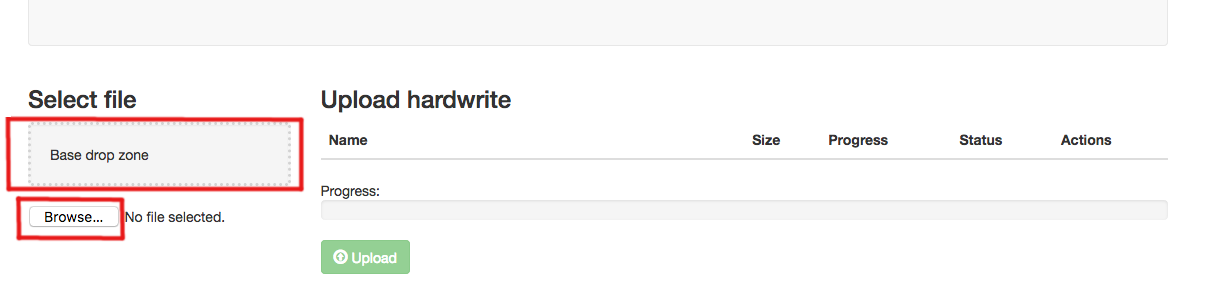
\includegraphics[width=0.6\textheight]{figures/select_sample_man.png}
    \caption{Экран выбора образца почерка}
    \label{fig:manpage:client_man:add_sample}
\end{figure}

\begin{figure}[ht]
    \centering
    \label{fig:manpage:client_man:upload_sample}
    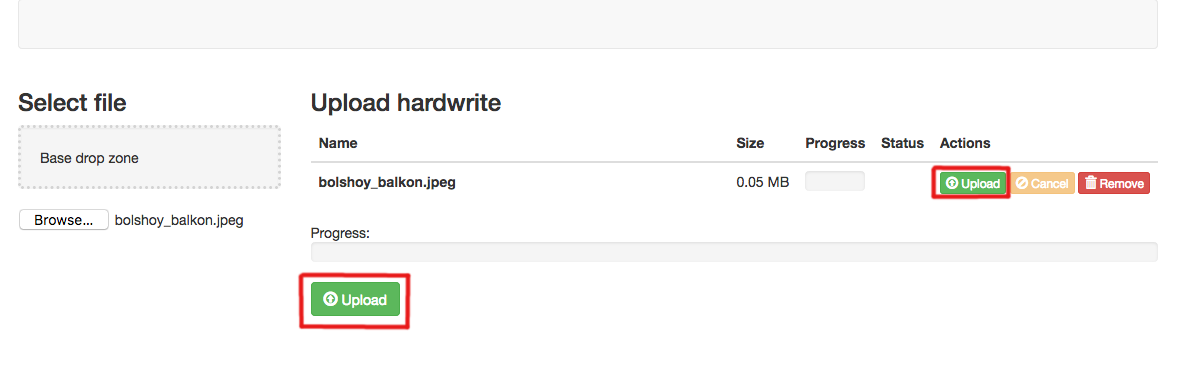
\includegraphics[width=0.6\textheight]{figures/upload_sample_man.png}
    \caption{Экран загрузки образца почерка}
    \label{fig:manpage:client_man:upload_sample}
\end{figure}

\subsubsection{Выделение признаков почерка}
\label{sec:manpage:client_man:features}
\begin{enumerate}
    \item[1)] авторизоваться в приложении;
    \item[2)] выбрать образец из ранее загруженных, нажав на кнопку <<Show>> около образца, рисунок ~\ref{fig:manpage:client_man:show_button};
    \item[3)] нажать кнопку <<Extract features>> и дождаться окончания обработки, рисунок ~\ref{fig:manpage:client_man:extract_features}.
\end{enumerate}

\begin{figure}[ht]
    \centering
    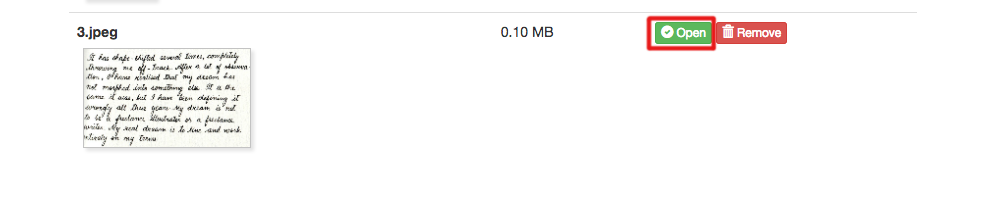
\includegraphics[width=0.6\textheight]{figures/samples_open.png}
    \caption{Выбор образца почерка}
    \label{fig:manpage:client_man:show_button}
\end{figure}

\begin{figure}[ht]
    \centering
    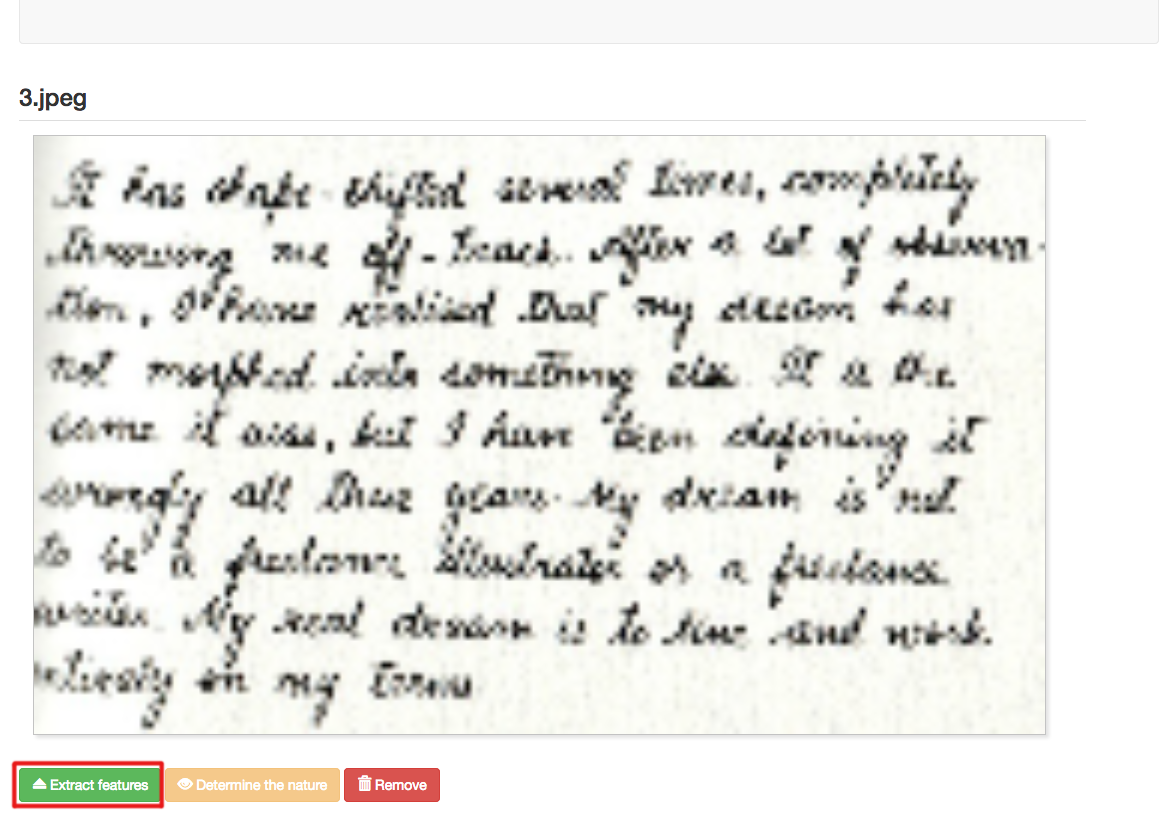
\includegraphics[width=0.3\textheight]{figures/extract_features.png}
    \caption{Экран просмотра образца почерка}
    \label{fig:manpage:client_man:extract_features}
\end{figure}

\subsubsection{Определение параметров личности}
\label{sec:manpage:client_man:determ_nature}
\begin{enumerate}
    \item[1)] авторизоваться в приложении;
    \item[2)] выбрать образец из ранее загруженных с выделенными признаками;
    \item[3)] нажать кнопку "Determinate" и дождаться окончания обработки, рисунок ~\ref{fig:manpage:client_man:determinate_nature}.
\end{enumerate}

\begin{figure}[ht]
    \centering
    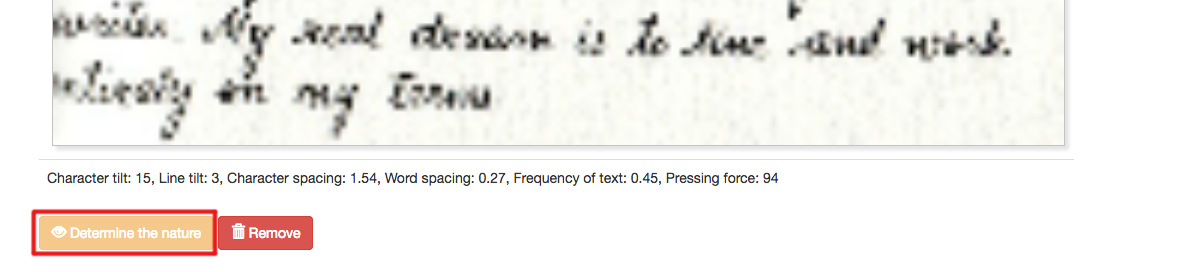
\includegraphics[width=0.3\textheight]{figures/determinate_nature.png}
    \caption{Определение признаков почерка}
    \label{fig:manpage:client_man:determinate_nature}
\end{figure}

\subsubsection{Удаление образца}
\label{sec:manpage:client_man:delete_sample}
\begin{enumerate}
    \item[1)] авторизоваться в приложении;
    \item[2)] нажать кнопку "Delete" рядом с изображением образца или на экране просмотра образца, рисунок ~\ref{fig:manpage:client_man:delete_sample};
    \item[3)] подтвердить удаление, рисунок.
\end{enumerate}

\begin{figure}[ht]
    \centering
    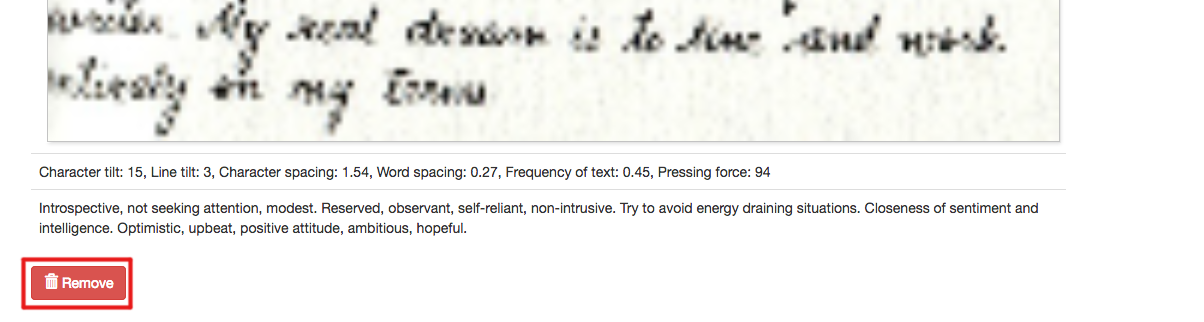
\includegraphics[width=0.3\textheight]{figures/delete_sample.png}
    \caption{Удаление образца почерка}
    \label{fig:manpage:client_man:delete_sample}
\end{figure}

